\documentclass[11pt,a4paper]{article}

% Packages
\usepackage[utf8]{inputenc}
\usepackage[T1]{fontenc}
\usepackage{amsmath,amssymb}
\usepackage{graphicx}
\usepackage{booktabs}
\usepackage{hyperref}
\usepackage[margin=1in]{geometry}
\usepackage{natbib}
\usepackage{caption}
\usepackage{subcaption}
\usepackage{multirow}
\usepackage{array}
\usepackage{xcolor}
\usepackage{algorithm}
\usepackage{algorithmic}
\usepackage{float}

\graphicspath{{../figures/}}

\hypersetup{
    colorlinks=true,
    linkcolor=blue,
    citecolor=blue,
    urlcolor=blue
}

\title{Critic Initialization, Gradient Stabilization, and Q-Value Regularization\\for Off-Policy Deep Reinforcement Learning}

\author{Tesfay Zemuy Gebrekidan, PhD\\
\texttt{tzemuy13@gmail.com}}

\date{March 2026}

\begin{document}

\maketitle

\begin{abstract}
We investigate five complementary techniques for improving off-policy deep reinforcement learning on hard-exploration continuous control tasks: (1)~\textbf{Reward-Range-Aware Initialization~(RWAI)} of critic last-layer weights and biases to the expected Q-value range; (2)~\textbf{Gradient Clipping~(GC)} via \texttt{clip\_grad\_norm\_} after each backward pass; (3)~\textbf{Adaptive Gradient Scaling~(AS)} of pre-tanh actor activations using running statistics; (4)~\textbf{Prioritized Experience Replay~(PER)} with importance-sampling-weighted loss; and (5)~\textbf{Q-Value Bounding~(QBound)} via two-stage hard clipping on critic TD targets and soft clipping on actor Q-values. We evaluate across a full combinatorial ablation: 3~off-policy algorithms (SAC, TD3, DDPG)~$\times$~2~environments (single and double inverted pendulum swing-up)~$\times$~$2^4 = 16$ combinations of \{RWAI~v2, PER, AS, QBound\}, plus PPO baselines, legacy RWAI~v1 experiments with vanilla baselines, and \texttt{norm\_reward=False} baselines, totaling \textbf{116~experiments}. QBound emerges as the most consistently beneficial technique for SAC, providing stable convergence (single:~$453.2/452.2$, double:~$455.7/455.7$ with PER). Notably, most of SAC's single-pendulum improvement ($312 \to 452.6$) comes from disabling reward normalization (required by QBound); QBound adds stability atop this ($+3.9$ final reward vs.\ \texttt{no\_norm\_reward} baseline). On double pendulum, standalone QBound matches the \texttt{no\_norm\_reward} baseline exactly; the benefit appears only with PER ($+47.0$ final). AS proves catastrophic for SAC without QBound (all pure-AS variants collapse), though QBound partially rescues AS-damaged SAC (AS+QBound single: 225, double: 421). AS partially rescues TD3 from exploration failure (single:~$8.7 \to 205$). RWAI~v2 improves SAC double pendulum (483 peak) but matches the \texttt{no\_norm\_reward} baseline on single; it destabilizes TD3. The best configurations combine QBound with PER for SAC ($453.6/453.5$ single, $455.7/455.7$ double) and PER with AS for TD3 double ($441.4/428.8$). These results demonstrate that technique effectiveness is strongly algorithm-dependent.
\end{abstract}

\section{Introduction}

Deep reinforcement learning algorithms that learn action-value (Q) functions---including SAC~\citep{haarnoja2018sac}, TD3~\citep{fujimoto2018td3}, and DDPG~\citep{lillicrap2016ddpg}---rely on value networks (critics) to estimate expected cumulative returns. These estimates drive policy updates: the actor chooses actions that maximize the value network's predictions. Consequently, the accuracy of value estimates, particularly during early training, has an outsized influence on learning dynamics.

Standard neural network initialization schemes (Xavier~\citep{glorot2010xavier}, Kaiming~\citep{he2015kaiming}, orthogonal~\citep{saxe2014orthogonal}) are designed to maintain gradient flow in deep networks. They center initial outputs near zero with bounded variance. While appropriate for classification and regression, this creates systematic bias for Q-value estimation when rewards are non-zero-centered.

This initialization mismatch is particularly problematic for off-policy algorithms because: (1)~bootstrap amplification propagates biased initial estimates through TD learning; (2)~entropy interaction in SAC makes the entropy bonus relatively larger when Q-values are underestimated; and (3)~persistent bias accumulates over the full training run unlike on-policy methods that re-estimate values each rollout.

Beyond initialization, off-policy algorithms face additional challenges: gradient instability from large TD errors, tanh saturation in deterministic actors, inefficient uniform replay sampling, and unconstrained Q-value divergence. We address these with five complementary techniques evaluated in a full combinatorial ablation across 116~experiments.

\section{Related Work}

\textbf{Overestimation bias.}~Thrun and Schwartz~\citep{thrun1993overestimation} first identified systematic overestimation in Q-learning. Fujimoto et al.~\citep{fujimoto2018td3} extended this to continuous control with TD3's clipped double-Q trick. Our work examines overestimation from initialization rather than the max operator.

\textbf{Network initialization.}~Glorot and Bengio~\citep{glorot2010xavier} proposed Xavier initialization; He et al.~\citep{he2015kaiming} developed Kaiming initialization for ReLU networks. These optimize gradient flow but do not consider output target magnitude.

\textbf{Conservative/Optimistic initialization.}~CQL~\citep{kumar2020cql} intentionally underestimates for offline RL. Optimistic initialization in tabular RL~\citep{sutton2018rl} encourages exploration. Our RWAI aims to \emph{match}, not artificially shift, the Q-value range.

\textbf{Prioritized Experience Replay.}~Schaul et al.~\citep{schaul2016per} introduced proportional prioritization with importance-sampling correction. We integrate PER with gradient clipping and Q-value bounding.

\textbf{Q-Value Bounding.}~Gebrekidan~\citep{gebrekidan2025qbound} introduced QBound, a method for constraining Q-value estimates to the theoretically achievable range using two-stage hard clipping on critic targets and soft (softplus) clipping on actor Q-values. We integrate QBound into our combinatorial ablation framework.

\textbf{Adaptive Gradient Scaling.}~Gebrekidan~\citep{gebrekidan2025as} identified gradient asymmetry and activation saturation as failure modes in deterministic actor networks and proposed an adaptive gradient scaling module to maintain pre-tanh activations in the high-gradient region. We evaluate this technique across SAC, TD3, and DDPG.

\textbf{Exploration noise.}~Hollenstein et al.~\citep{hollenstein2022noise} showed OU noise outperforms Gaussian for swing-up tasks. Eberhard et al.~\citep{eberhard2023pink} confirmed temporally correlated noise advantages. We adopt OU noise for TD3 and DDPG.

\section{Method}

\subsection{Problem Setup}

Consider an environment with reward $r(s,a) \in [r_{\min}, r_{\max}]$, discount $\gamma$, and maximum episode length $H$. For dense rewards, the Q-value range is:
\begin{equation}
Q_{\min} = r_{\min} \cdot \frac{1-\gamma^H}{1-\gamma}, \quad Q_{\max} = r_{\max} \cdot \frac{1-\gamma^H}{1-\gamma}
\end{equation}

\subsection{Reward-Range-Aware Initialization (RWAI)}

\textbf{RWAI~v1 (bias-only):} Set the critic's last linear layer bias to $Q_{\text{mid}} = (Q_{\min} + Q_{\max})/2$, while leaving the Kaiming-initialized weights unchanged:
\begin{equation}
b \leftarrow Q_{\text{mid}}, \qquad \mathbf{W} \leftarrow \mathbf{W}_{\text{Kaiming}}
\end{equation}
This shifts the output distribution to the correct center but preserves the default (small) output variance, so all state-action pairs initially produce similar Q-estimates near $Q_{\text{mid}}$.

\textbf{RWAI~v2 (scaled weights):} In addition to centering, the last-layer weights are scaled so that the output standard deviation spans the Q-value range. Given the target std $\sigma_{\text{target}} = Q_{\text{range}}/4$ (so $\pm 2\sigma$ covers $[Q_{\min}, Q_{\max}]$):
\begin{align}
s &= \min\!\left(\frac{\sigma_{\text{target}}}{\sigma_{\text{current}}},\; 100\right) \\
\mathbf{W} &\leftarrow s \cdot \mathbf{W}_{\text{Kaiming}} \\
b &\leftarrow s \cdot b_{\text{Kaiming}} + Q_{\text{mid}} \cdot (1 - s)
\end{align}
where $\sigma_{\text{current}}$ is measured empirically by passing random inputs through the hidden layers. The scale cap of $100\times$ prevents extreme gradient amplification. This gives different state-action pairs meaningfully different initial Q-estimates across the full $[Q_{\min}, Q_{\max}]$ range, rather than all concentrating near $Q_{\text{mid}}$.

Both variants require \texttt{norm\_reward=False} so that the raw Q-value range matches the training targets. With reward normalization (VecNormalize), the effective Q-range shrinks to $\approx[0, 10]$, causing $5$--$50\times$ overestimation (Table~\ref{tab:rwai_v1}).

\subsection{Q-Range Computation}

\begin{table}[h]
\centering
\caption{Q-value ranges for our environments ($r_{\min}=-0.5$, $r_{\max}=1.0$, $\gamma=0.99$).}
\begin{tabular}{lcccccc}
\toprule
Environment & $H$ & $Q_{\min}$ & $Q_{\max}$ & $Q_{\text{mid}}$ \\
\midrule
Single pendulum & 500 & $-49.67$ & $99.34$ & $24.84$ \\
Double pendulum & 1000 & $-50.00$ & $100.00$ & $25.00$ \\
\bottomrule
\end{tabular}
\label{tab:qrange}
\end{table}

\subsection{Gradient Clipping (GC)}

SB3~2.7.1's SAC, TD3, and DDPG do not natively support \texttt{max\_grad\_norm}. We subclass each algorithm and insert \texttt{clip\_grad\_norm\_()} after each \texttt{backward()} call, clipping both critic and actor gradients to a maximum $L_2$ norm of~1.0. All off-policy experiments use GC as standard.

\subsection{Adaptive Gradient Scaling (AS)~\citep{gebrekidan2025as}}

An \textbf{AdaptiveGradientScaler} module is placed before the tanh nonlinearity. It tracks running mean $\mu$ and standard deviation $\sigma$ of pre-tanh activations using EMA (decay 0.99), then linearly maps $[\mu - k\sigma, \mu + k\sigma]$ to $[-t, +t]$, where $k=2.5$ and target range $t=2.0$:
\begin{equation}
x_{\text{scaled}} = \frac{x - \mu}{k \cdot \sigma} \cdot t
\end{equation}

\subsection{Prioritized Experience Replay (PER)}

Transitions are sampled proportional to their TD error with exponent $\alpha=0.6$. Importance-sampling weights $w_i = (N \cdot P(i))^{-\beta}$ correct the bias, with $\beta$ annealed linearly from 0.4 to 1.0. A sum-tree data structure enables $O(\log n)$ sampling.

\subsection{Q-Value Bounding (QBound)~\citep{gebrekidan2025qbound}}

\textbf{Critic (hard clipping):}
\begin{align}
\hat{Q}(s',a') &= \text{clamp}(Q_{\text{target}}(s',a'),\; Q_{\min},\; Q_{\max}) \\
y &= \text{clamp}(r + \gamma \hat{Q}(s',a'),\; Q_{\min},\; Q_{\max})
\end{align}

\textbf{Actor (soft clipping):} Softplus-based ($\beta=5.0$) smooth enforcement of bounds preserves gradient flow:
\begin{equation}
Q_{\text{clip}} = Q_{\max} - \text{softplus}\!\left(Q_{\max} - \left(Q_{\min} + \text{softplus}(Q - Q_{\min}, \beta)\right), \beta\right)
\end{equation}

\section{Experimental Setup}

\subsection{Environments}

\textbf{Single Pendulum Swing-Up} (\texttt{CartPoleSwingUp-v0}): A cart (mass $M=1.0$\,kg) on a 1D track with a pole (mass $m=0.1$\,kg, half-length $l=0.5$\,m) attached via a free hinge. The pole starts hanging down ($\theta=\pi$) and must be swung up ($\theta=0$) and balanced. 5D observation $[x, \sin\theta, \cos\theta, \dot{x}, \dot{\theta}]$, 1D continuous action $\in [-1,1]$ scaled by $F_{\max}=10$\,N, 500-step episodes.

The equations of motion are derived from the Euler--Lagrange equations:
\begin{align}
(M + m)\ddot{x} + ml\ddot{\theta}\cos\theta - ml\dot{\theta}^2\sin\theta &= F - \mu\dot{x} \\
ml\ddot{x}\cos\theta + ml^2\ddot{\theta} - mgl\sin\theta &= 0
\end{align}
where $\mu=0.1$ is the cart friction coefficient. These are solved analytically for $\ddot{x}$ and $\ddot{\theta}$ at each substep.

\textbf{Double Pendulum Swing-Up} (\texttt{DoubleCartPoleSwingUp-v0}): Two identical poles ($m_1=m_2=0.1$\,kg, $l_1=l_2=0.5$\,m half-length) connected in series on the same cart. 8D observation $[x, \sin\theta_1, \cos\theta_1, \sin\theta_2, \cos\theta_2, \dot{x}, \dot{\theta}_1, \dot{\theta}_2]$, 1000-step episodes. The dynamics are governed by a $3\times 3$ mass matrix $\mathbf{M}(\mathbf{q})\ddot{\mathbf{q}} = \mathbf{f}(\mathbf{q}, \dot{\mathbf{q}}, u)$ for generalized coordinates $\mathbf{q} = [x, \theta_1, \theta_2]$, including Coriolis, centrifugal, and gravitational terms, solved via \texttt{np.linalg.solve} at each substep.

Both environments use 4th-order Runge--Kutta (RK4) integration with sub-stepping (2 steps single, 4 steps double) for numerical stability. Angles are represented as $\sin/\cos$ pairs to avoid discontinuity at $\pm\pi$. The cart terminates at $|x| > 2.4$\,m.

\textbf{Reward (single pendulum):}
\begin{equation}
r = \underbrace{\tfrac{\cos\theta + 1}{2}}_{\text{uprightness}} - \underbrace{0.01\,x^2}_{\text{cart}} - \underbrace{0.001\,a^2}_{\text{control}} - \underbrace{0.002\,u^4\dot{\theta}^2}_{\text{velocity}}
\end{equation}
where $u = (\cos\theta+1)/2$ is the uprightness factor. The smooth $u^4$ activation avoids reward discontinuity near the upright position. The double pendulum reward uses a weighted combination of individual pole uprightness ($0.4$ each) and normalized tip height ($0.2$), with cart penalty coefficient $0.005$. Reward range: $[-0.5, 1.0]$ per step for both environments.

\subsection{Algorithms and Experiment Matrix}

The full matrix comprises \textbf{116 experiments}: 3~off-policy algorithms $\times$ 2~environments $\times$ 16~combinations of \{RWAI~v2, PER, AS, QBound\} $=$ 96, plus 2~PPO baselines, 6~legacy RWAI~v1, 6~vanilla baselines (for v1 comparison), and 6~\texttt{norm\_reward=False} baselines.

\begin{table}[h]
\centering
\caption{Algorithm configurations.}
\begin{tabular}{lclll}
\toprule
Algorithm & Critics & Exploration & Key Property \\
\midrule
PPO & 1 (value fn) & SDE + 4 parallel envs & On-policy control \\
SAC & 2 (clipped) & Entropy + SDE & Max entropy objective \\
TD3 & 2 (clipped) & OU noise & Delayed updates \\
DDPG & 1 & OU noise & No double-Q \\
\bottomrule
\end{tabular}
\end{table}

\subsection{Shared Configuration}

All experiments: 500K timesteps, seed 42, VecNormalize observations, evaluation every 10K steps (10 episodes, deterministic). Off-policy: lr=$7.3 \times 10^{-4}$, buffer 50K, batch 128, $\gamma=0.99$, $\tau=0.02$, network $[64, 64]$ MLP, \texttt{max\_grad\_norm}$=1.0$.

\section{Results}

\subsection{RWAI v1 Legacy Results}

\begin{table}[h]
\centering
\caption{RWAI v1 results (with VecNormalize confound). Best / Final mean eval rewards. These experiments use vanilla SB3 classes (no gradient clipping) with \texttt{norm\_reward=True} to reproduce the original confound conditions.}
\begin{tabular}{llrrrr}
\toprule
Algorithm & Env & Default Best & Default Final & RWAI v1 Best & RWAI v1 Final \\
\midrule
SAC & Single & 375.9 & 364.0 & 179.5 & $-0.3$ \\
SAC & Double & 457.0 & 416.6 & 263.4 & 19.4 \\
TD3 & Single & 8.7 & 8.7 & 272.4 & 43.2 \\
TD3 & Double & 449.9 & 120.1 & 306.9 & $-6.5$ \\
DDPG & Single & 284.6 & 181.5 & 258.5 & 214.3 \\
DDPG & Double & 437.4 & 231.8 & 407.0 & 286.5 \\
\bottomrule
\end{tabular}
\label{tab:rwai_v1}
\end{table}

RWAI v1 reveals a critical confound: setting critic bias to $Q_{\text{mid}} \approx 50$ while VecNormalize rescales rewards to $\approx[0, 10]$ causes 5--50$\times$ overestimation. TD3's temporary rescue (8.7$\to$272.4 single, 449.9$\to$306.9 double) before collapse confirms that the exploration failure is due to conservative Q-estimation, not algorithmic incapacity. DDPG shows a moderate positive effect on final reward (181.5$\to$214.3 single, 231.8$\to$286.5 double) despite lower peak performance, suggesting greater robustness to Q-value misalignment.

\begin{figure}[H]
\centering
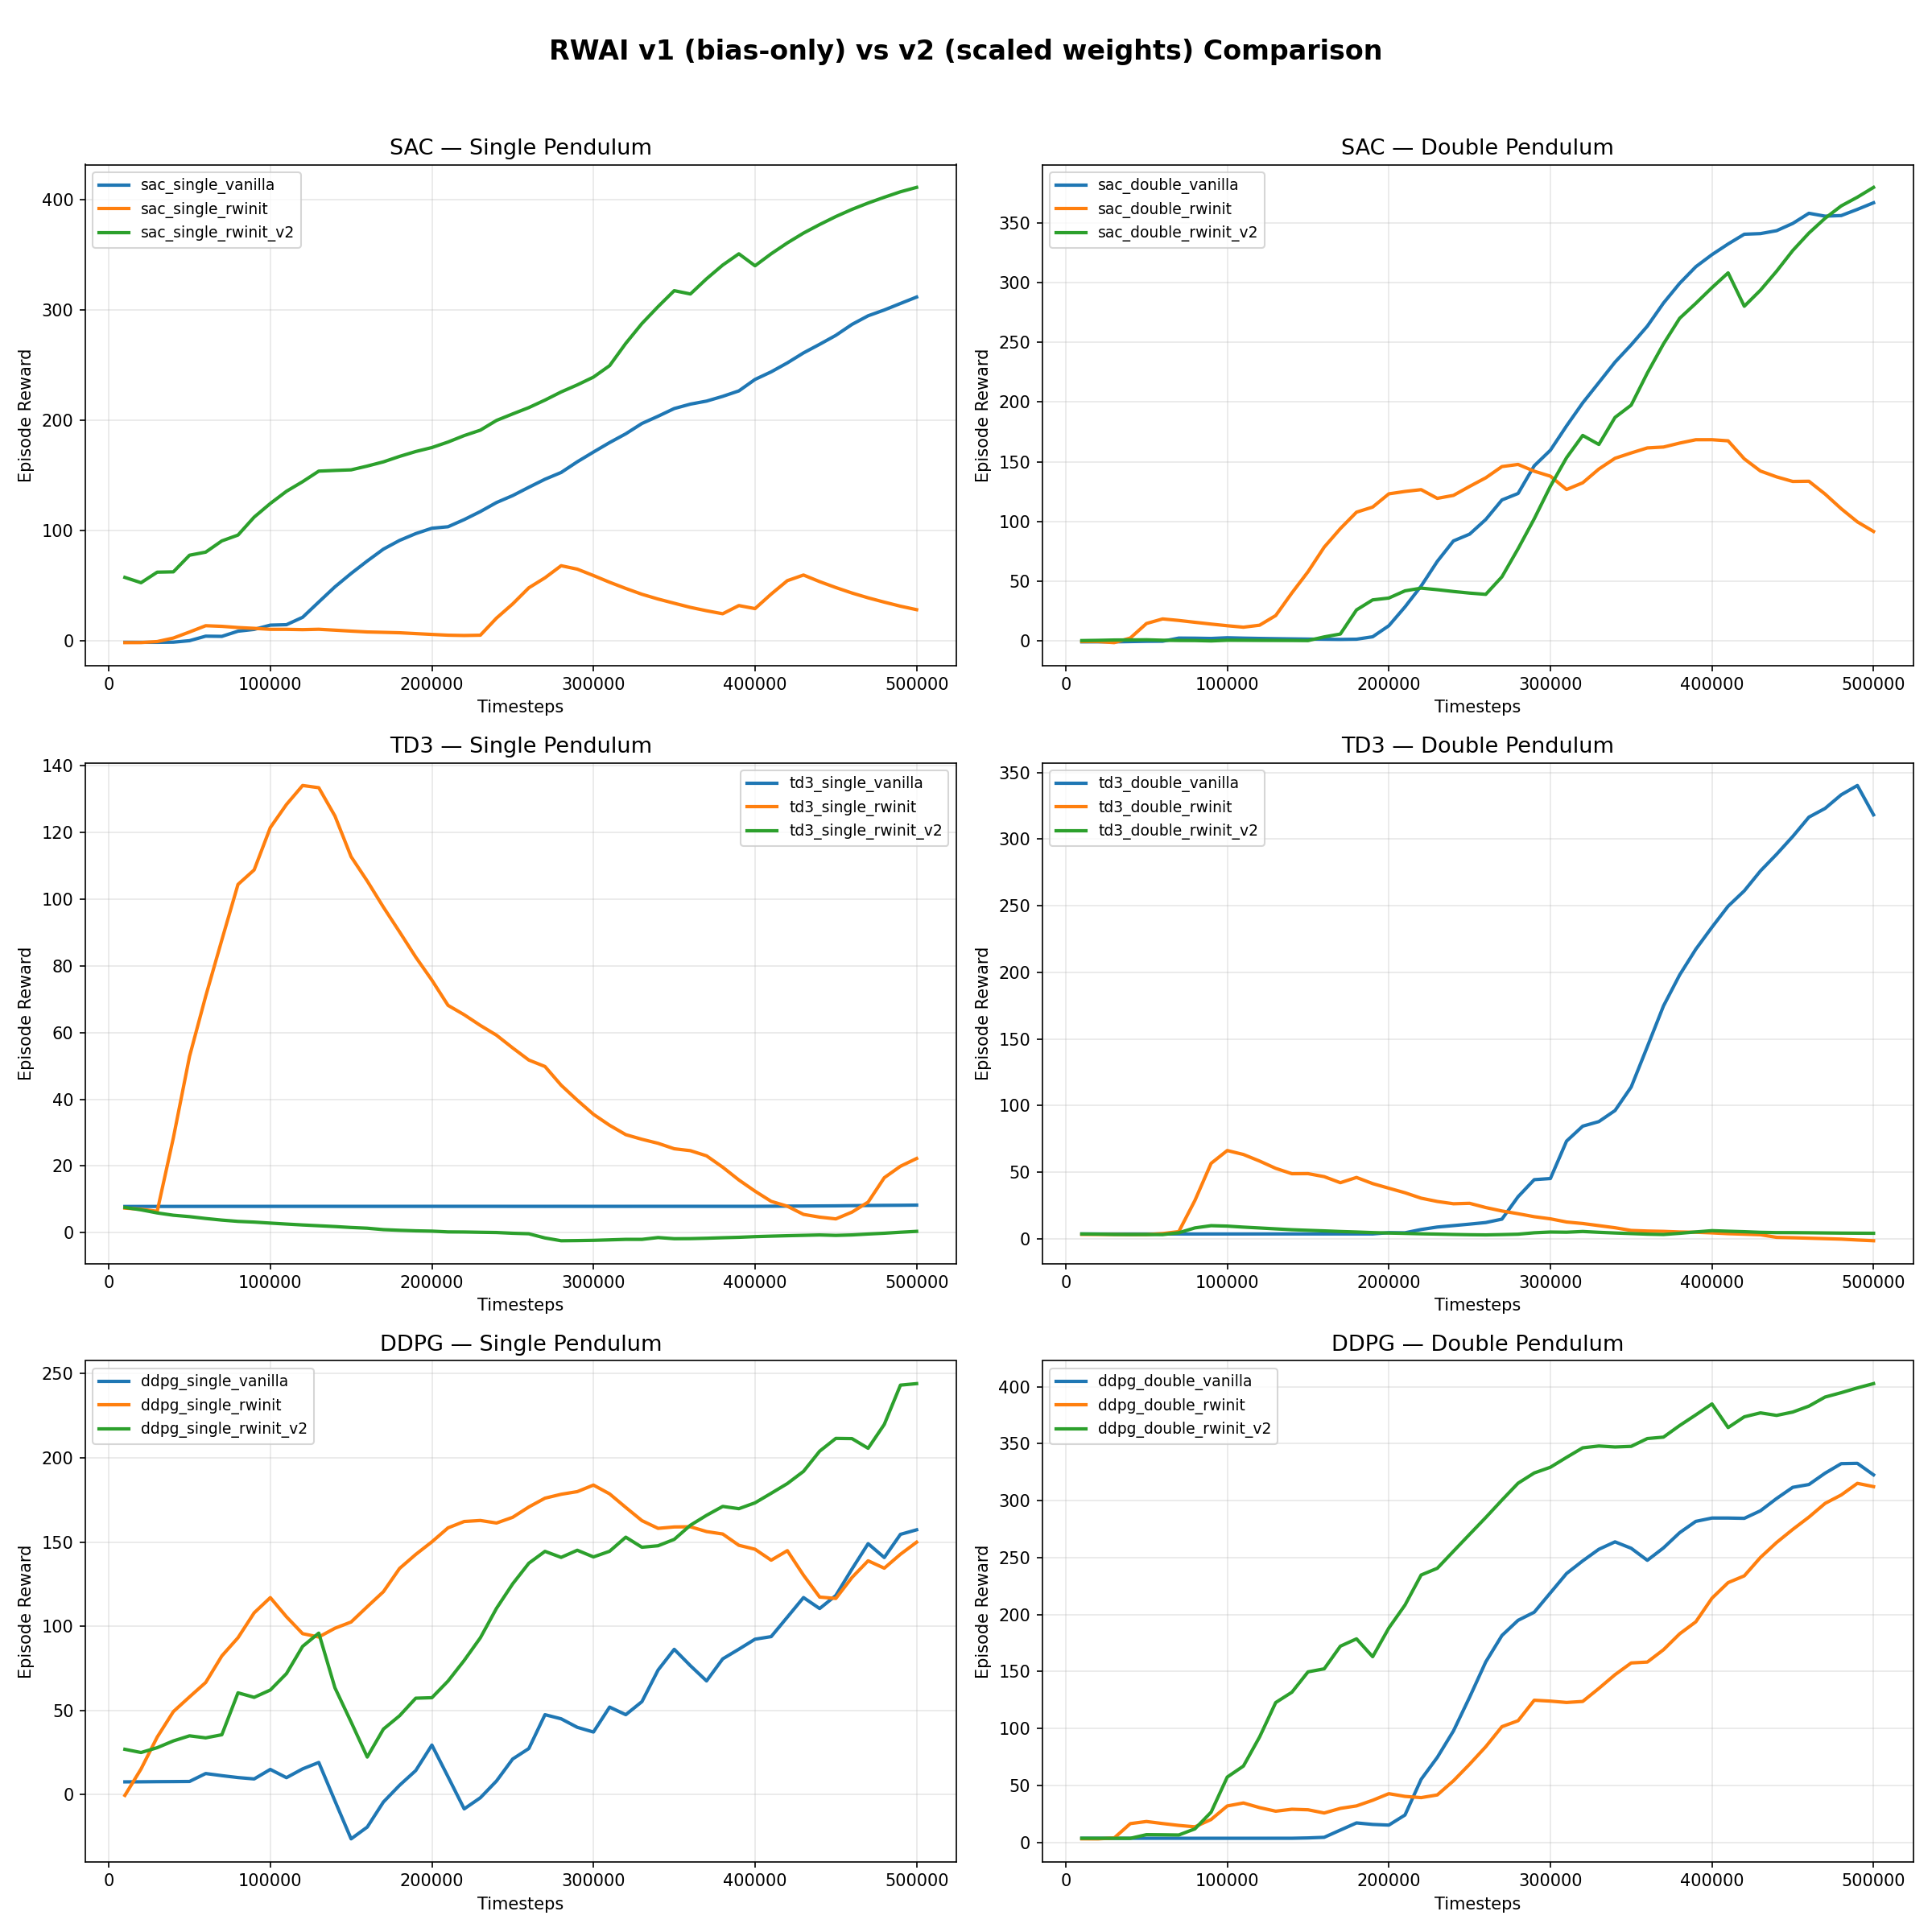
\includegraphics[width=\textwidth]{rwai_v1_vs_v2_comparison.png}
\caption{RWAI v1 vs v2 comparison across SAC, TD3, and DDPG on single and double pendulum environments. v1 (orange) shows characteristic collapse patterns under VecNormalize confound; v2 (green) with \texttt{norm\_reward=False} shows improved stability for SAC and DDPG but continued instability for TD3.}
\label{fig:v1_vs_v2}
\end{figure}

\subsection{Complete Combinatorial Results}

\subsubsection{SAC Results}

\begin{table}[h]
\centering
\caption{SAC: Best / Final mean eval rewards across all technique combinations.}
\small
\begin{tabular}{lcccc}
\toprule
Variant & Single Best & Single Final & Double Best & Double Final \\
\midrule
Baseline (GC, norm\_reward) & 312.4 & 312.4 & 434.5 & 369.9 \\
no\_norm\_reward baseline & 452.6 & 448.3 & 452.0 & 408.7 \\
RWAI v2 & 452.6 & 446.9 & \textbf{482.9} & 453.7 \\
PER & 453.0 & 388.7 & 423.5 & 371.4 \\
\textbf{QBound} & \textbf{453.2} & \textbf{452.2} & 452.0 & 408.7 \\
RWAI v2 + PER & 454.4 & 453.3 & 456.1 & 444.7 \\
\textbf{PER + QBound} & 453.6 & \textbf{453.5} & 455.7 & \textbf{455.7} \\
RWAI v2 + PER + QBound & 454.4 & 453.3 & 463.1 & 424.7 \\
\midrule
\multicolumn{5}{l}{\emph{AS-containing variants (AS disrupts SAC's log-probability; QBound partially rescues)}} \\
AS & 8.0 & 4.9 & 3.2 & 3.2 \\
AS + QBound & 225.4 & 171.8 & 420.7 & 375.8 \\
PER + AS & 101.2 & 3.3 & 118.2 & 67.0 \\
PER + AS + QBound & 197.2 & 133.4 & 434.3 & 405.5 \\
\bottomrule
\end{tabular}
\label{tab:sac_results}
\end{table}

\textbf{Key findings:} QBound provides the most stable SAC performance. Against the fair \texttt{no\_norm\_reward} baseline (452.6/448.3 single), QBound adds modest stability ($+3.9$ final), while PER + QBound achieves the highest stable finals (453.5/455.7). AS without QBound is catastrophic for SAC (all variants $<120$); QBound partially rescues AS-damaged SAC (single: 225.4, double: 420.7).

\begin{figure}[H]
\centering
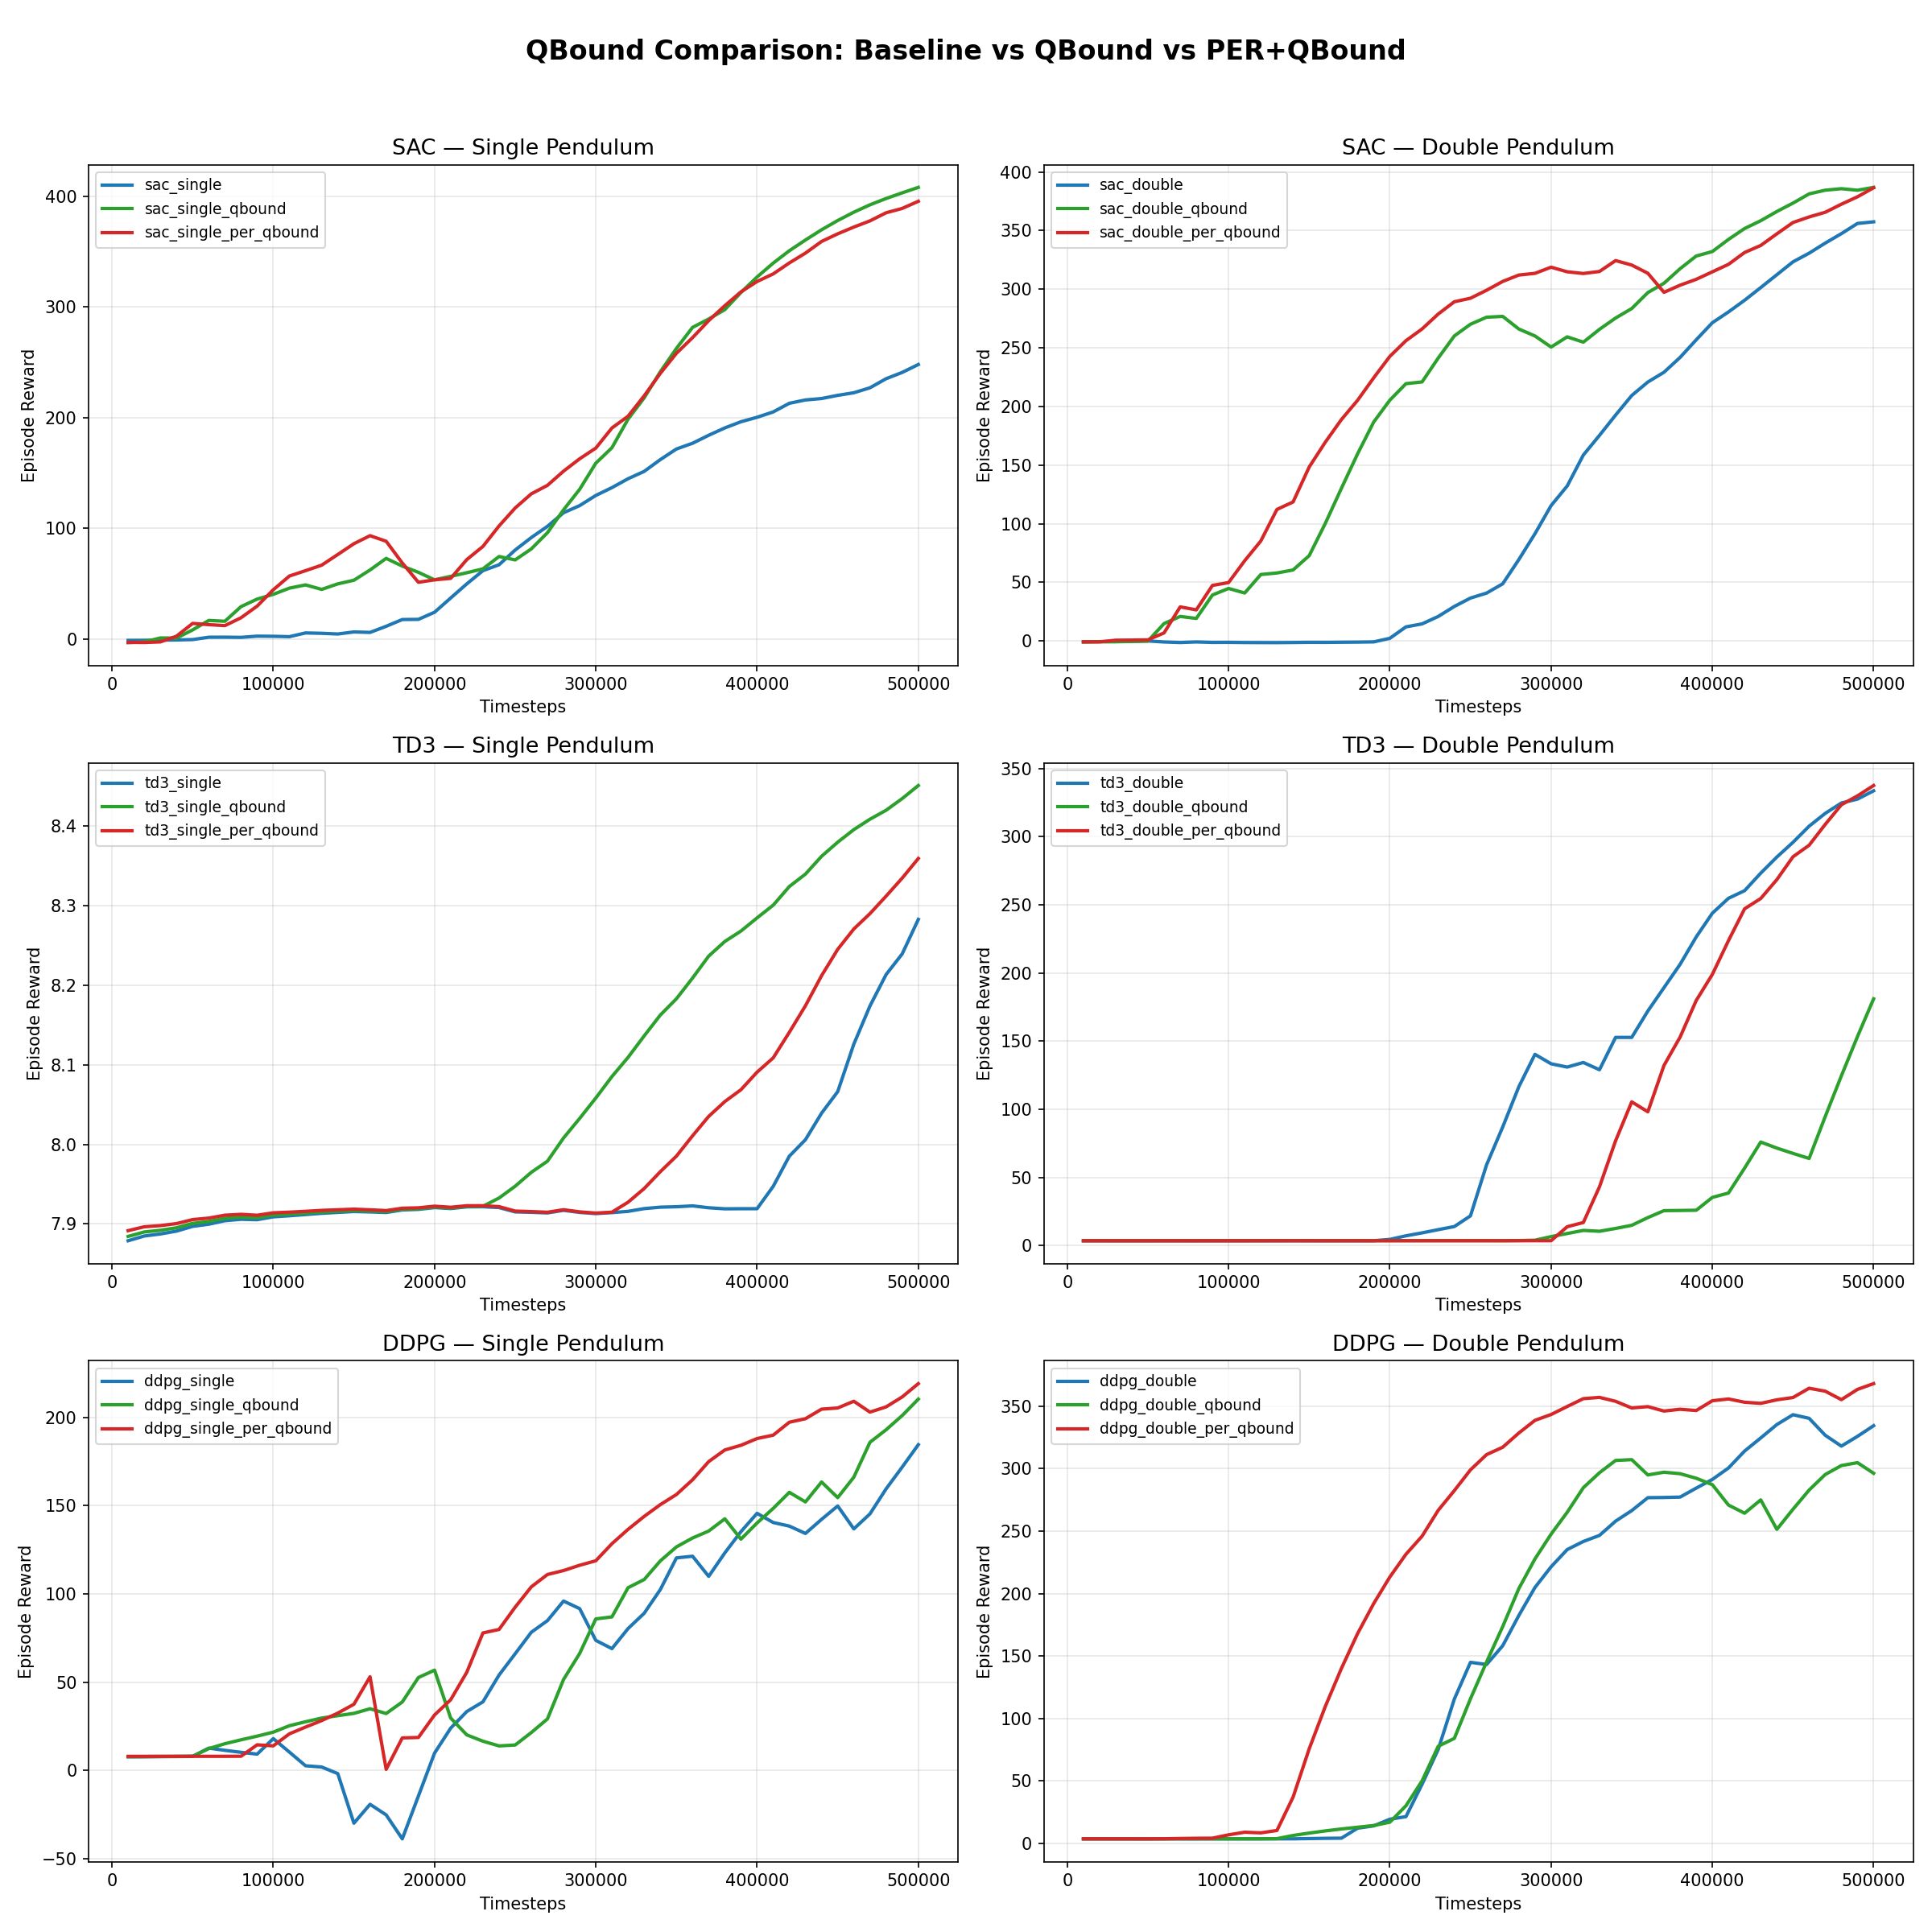
\includegraphics[width=\textwidth]{qbound_comparison.png}
\caption{QBound comparison: baseline (blue) vs QBound (green) vs PER+QBound (red). QBound dramatically improves SAC on both environments while having minimal effect on TD3's single-pendulum exploration failure. PER+QBound provides the most stable SAC performance.}
\label{fig:qbound}
\end{figure}

\begin{figure}[H]
\centering
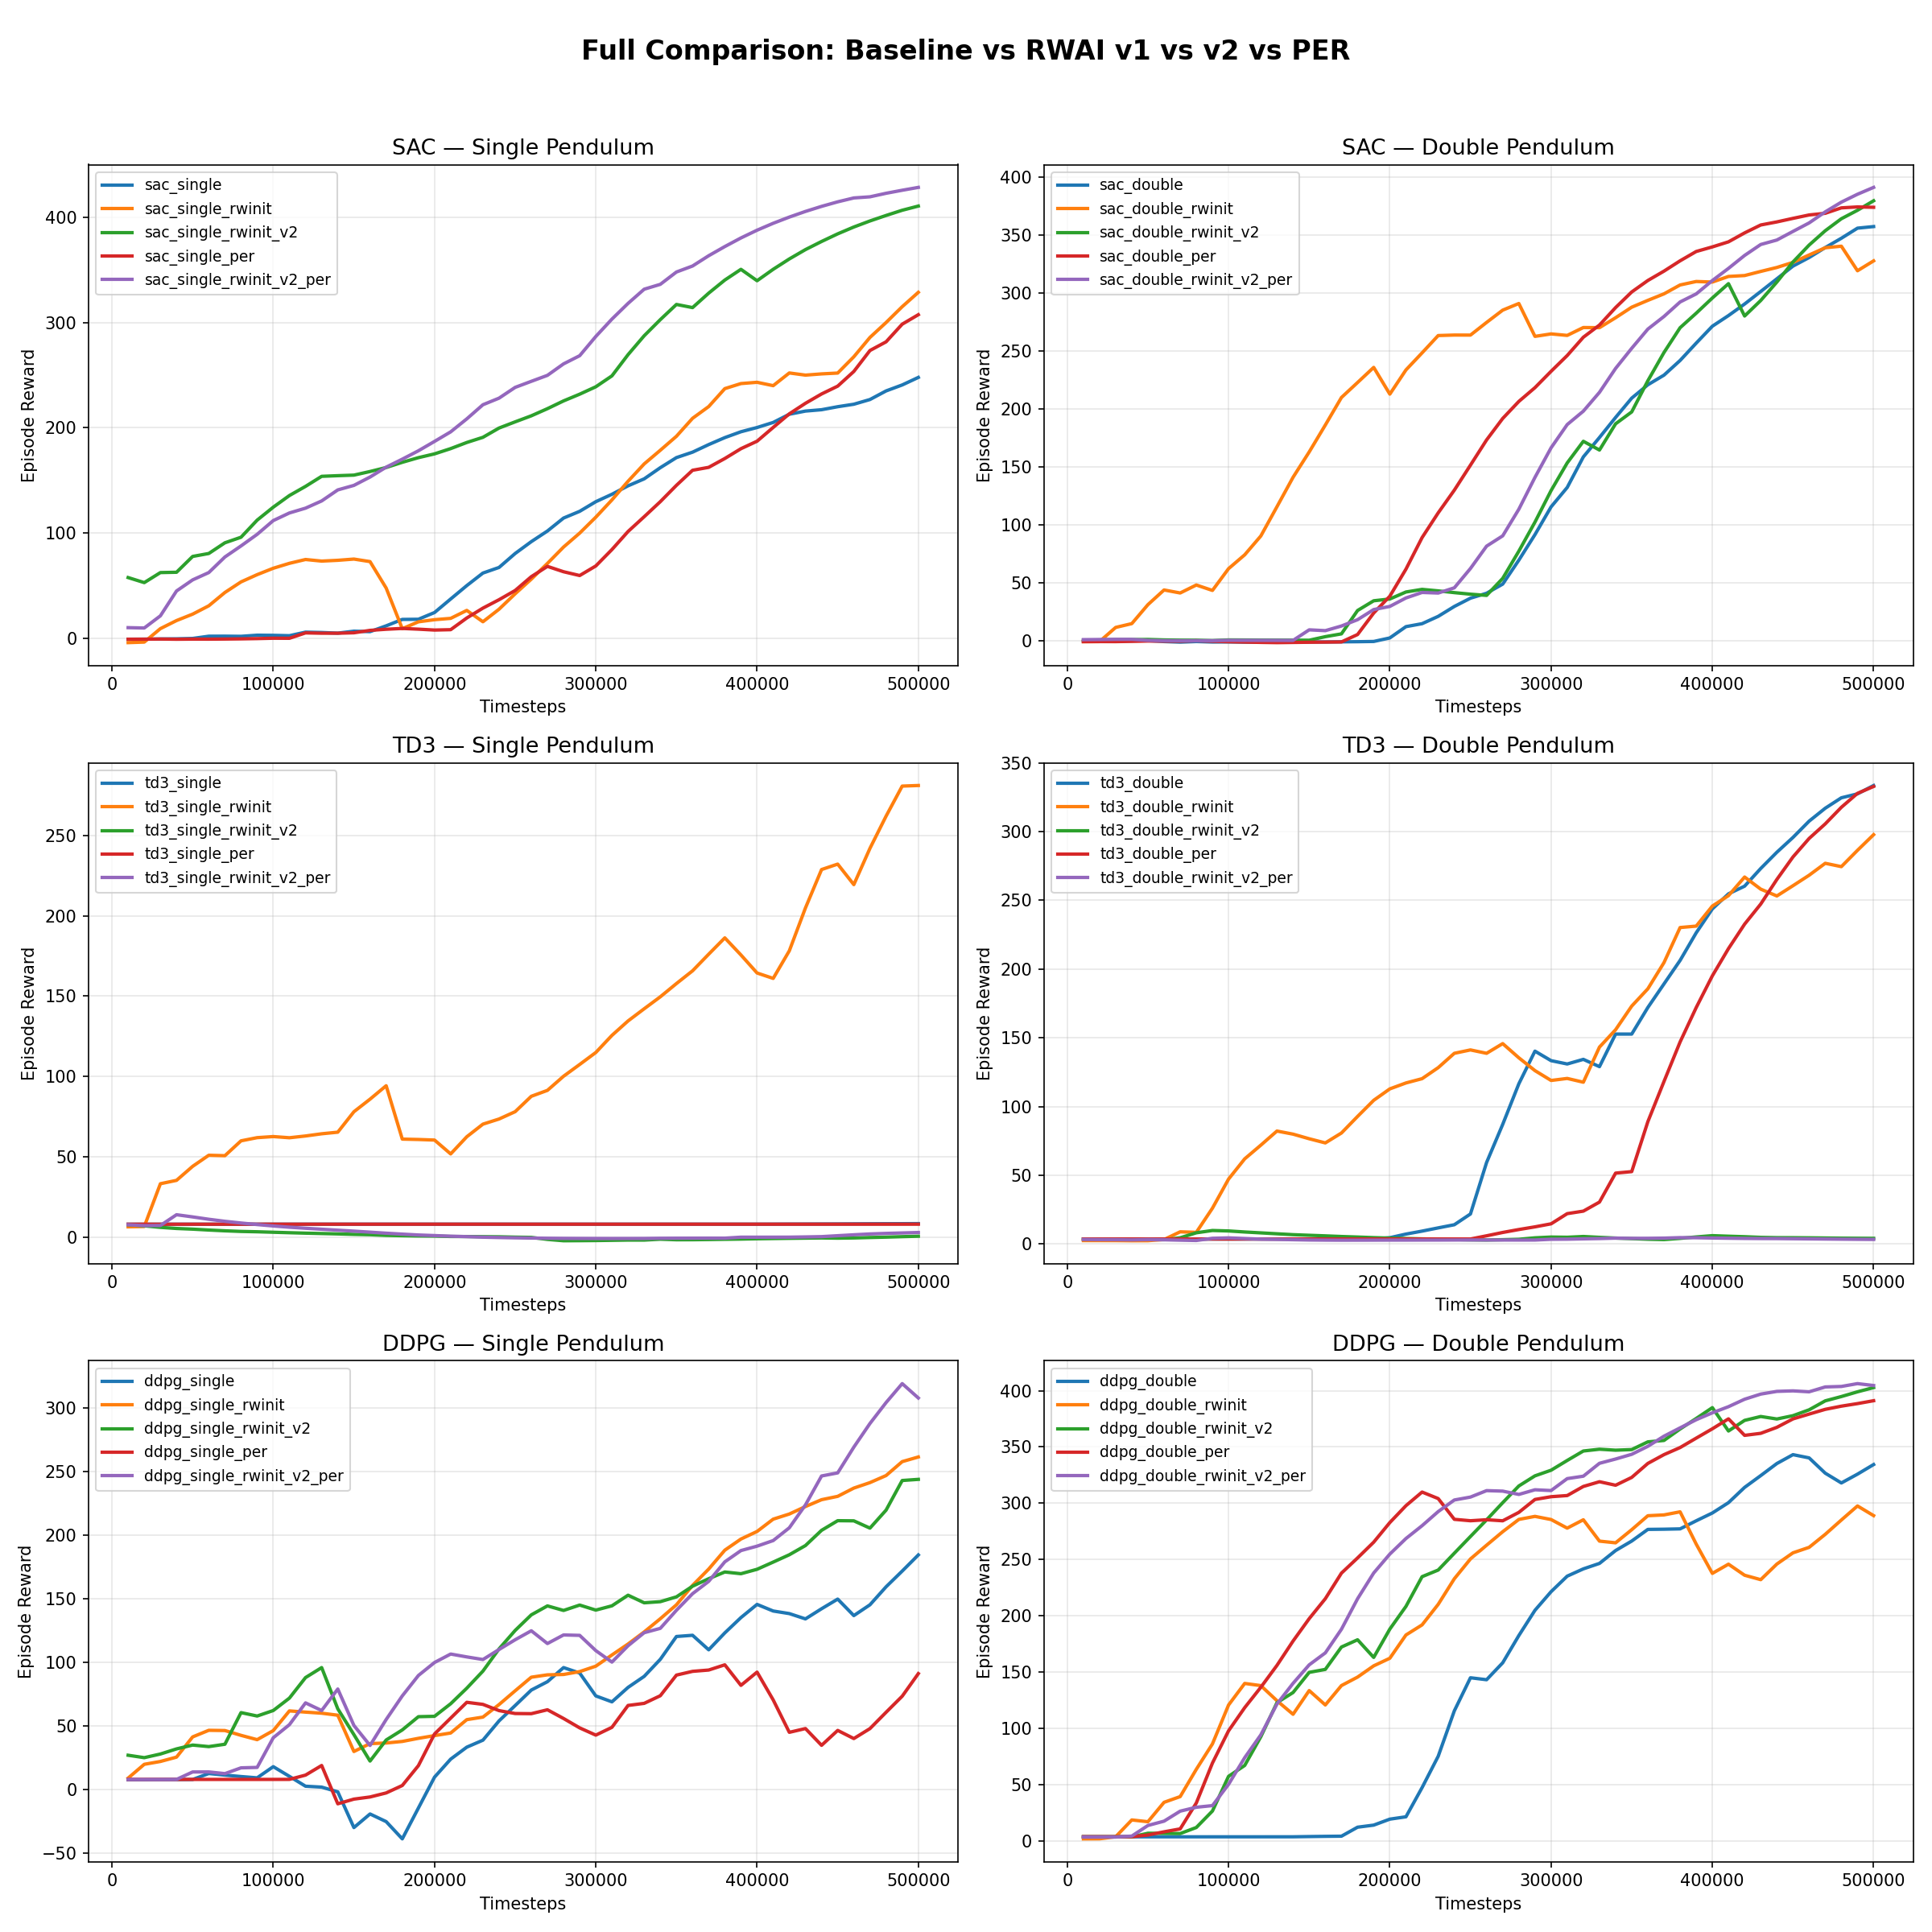
\includegraphics[width=\textwidth]{full_comparison.png}
\caption{Full comparison: baseline vs RWAI v1 vs RWAI v2 vs PER variants. RWAI v2 (green) improves SAC over baseline (blue) and avoids the v1 collapse pattern. PER+RWAI v2 (purple) achieves the highest SAC single peak (454.4).}
\label{fig:full_comparison}
\end{figure}

\subsubsection{TD3 Results}

\begin{table}[h]
\centering
\caption{TD3: Best / Final mean eval rewards (selected variants).}
\small
\begin{tabular}{lcccc}
\toprule
Variant & Single Best & Single Final & Double Best & Double Final \\
\midrule
Baseline (GC, norm\_reward) & 8.7 & 8.7 & 414.2 & 388.3 \\
RWAI v2 & 7.6 & 2.8 & 40.9 & 3.6 \\
AS & 205.4 & 173.9 & 409.3 & 390.7 \\
QBound & 8.6 & 8.6 & 429.9 & 429.9 \\
\textbf{PER + AS} & \textbf{292.5} & \textbf{269.5} & 441.4 & \textbf{428.8} \\
PER + QBound & 8.6 & 8.6 & \textbf{457.1} & 405.8 \\
RWAI v2 + PER + AS & 24.3 & $-0.3$ & 413.5 & 412.8 \\
\bottomrule
\end{tabular}
\label{tab:td3_results}
\end{table}

\textbf{Key findings:} TD3 single remains largely unsolvable. Only AS provides partial rescue ($8.7 \to 205$, $293$ with PER). RWAI v2 is destructive for TD3. PER + AS is the best TD3 combination.

\begin{figure}[H]
\centering
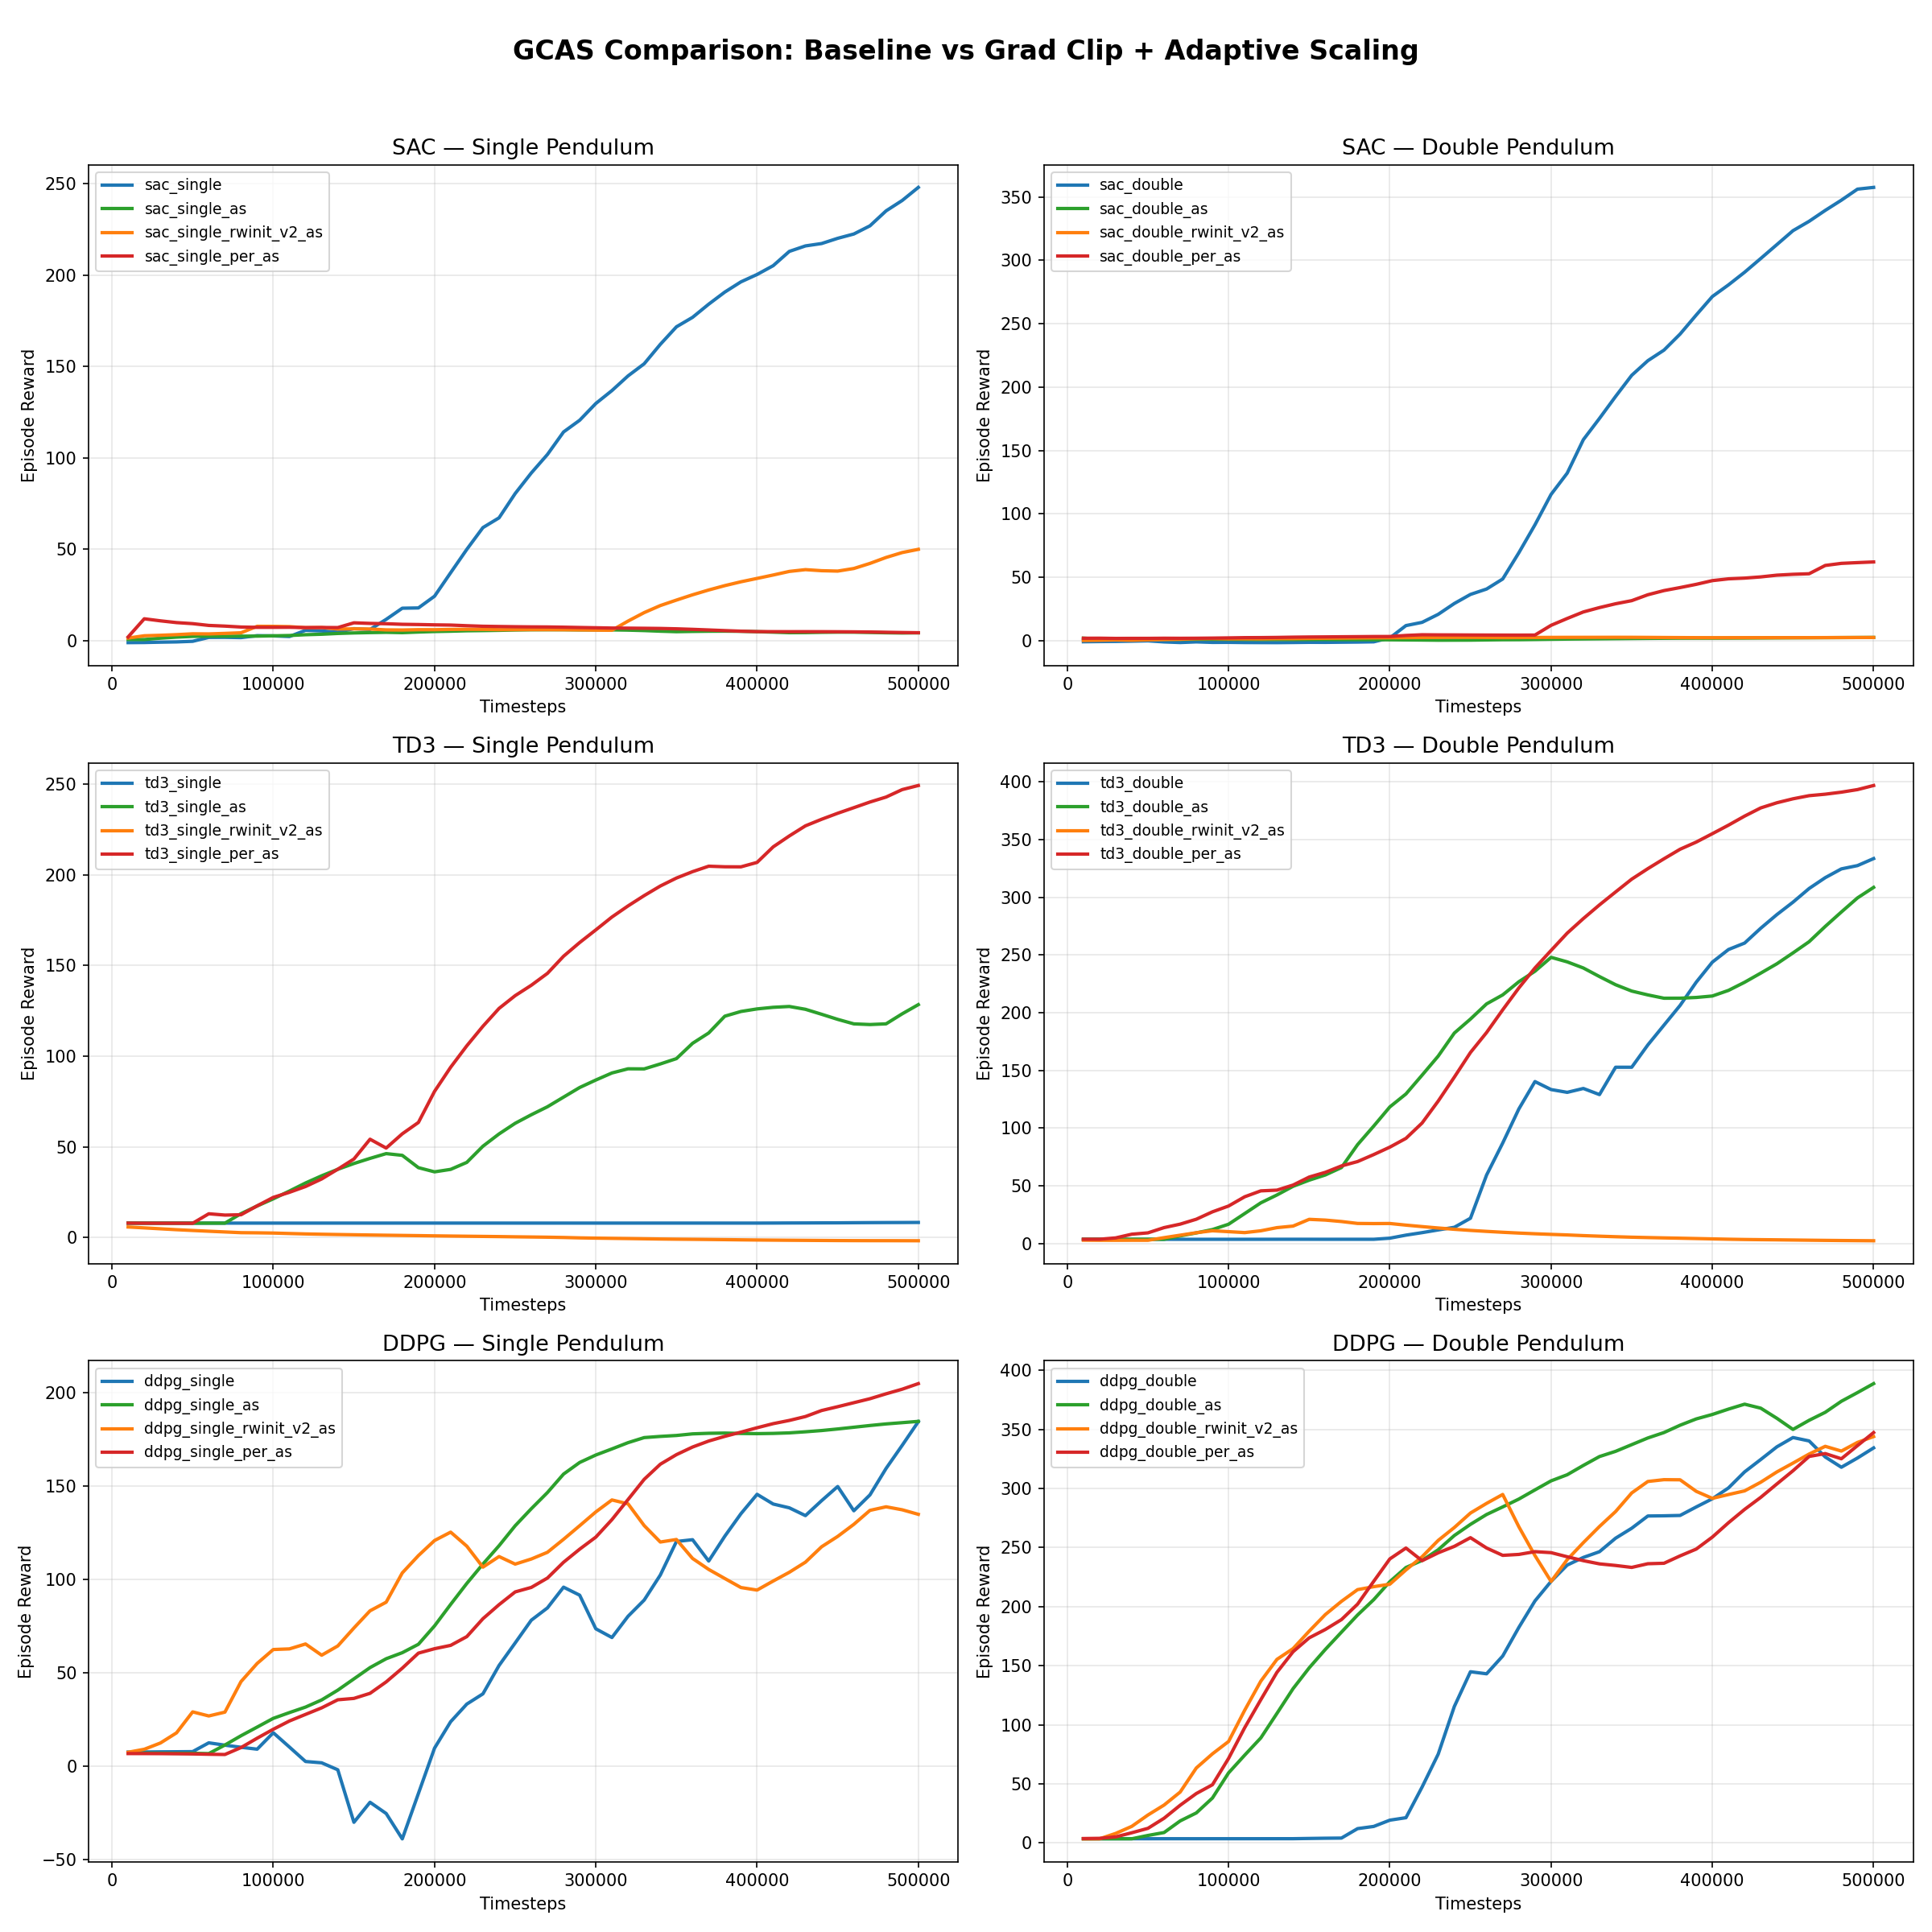
\includegraphics[width=\textwidth]{gcas_comparison.png}
\caption{Adaptive Gradient Scaling (AS) comparison: baseline (blue) vs AS (green) vs RWAI+AS (orange) vs PER+AS (red). AS partially rescues TD3 single from exploration failure but is catastrophic for SAC. PER+AS (red) achieves the best TD3 single-pendulum performance.}
\label{fig:gcas}
\end{figure}

\subsubsection{DDPG Results}

\begin{table}[h]
\centering
\caption{DDPG: Best / Final mean eval rewards (selected variants).}
\small
\begin{tabular}{lcccc}
\toprule
Variant & Single Best & Single Final & Double Best & Double Final \\
\midrule
Baseline (GC, norm\_reward) & 298.8 & 298.8 & \textbf{478.6} & 411.2 \\
RWAI v2 & \textbf{453.0} & 252.2 & 472.4 & 436.6 \\
AS & 245.5 & 190.9 & 457.9 & \textbf{457.1} \\
RWAI v2 + PER & 455.4 & 206.2 & 459.0 & 389.3 \\
PER + AS & 251.0 & 231.8 & 446.7 & 446.7 \\
RWAI v2 + PER + AS & 242.7 & 190.1 & 448.5 & 448.5 \\
\bottomrule
\end{tabular}
\label{tab:ddpg_results}
\end{table}

\textbf{Key findings:} RWAI v2 achieves highest single-pendulum peak (453.0) but with instability (final: 252.2). AS provides the most stable double performance (457.9/457.1). DDPG avoids the catastrophic failures seen with SAC+AS and TD3+RWAI v2, though its performance varies substantially across configurations.

\subsubsection{Cross-Algorithm Best Performers}

\begin{table}[h]
\centering
\caption{Top configurations by environment.}
\begin{tabular}{llcc}
\toprule
Environment & Configuration & Best & Final \\
\midrule
Single & SAC + RWAI v2 + PER & 454.4 & 453.3 \\
Single & SAC + PER + QBound & 453.6 & 453.5 \\
Single & SAC + QBound & 453.2 & 452.2 \\
Double & SAC + RWAI v2 & 482.9 & 453.7 \\
Double & SAC + PER + QBound & 455.7 & 455.7 \\
Double & DDPG + AS & 457.9 & 457.1 \\
\bottomrule
\end{tabular}
\label{tab:best}
\end{table}

PPO baselines: $450.2/439.0$ (single), $488.0/458.7$ (double). PPO establishes the on-policy performance ceiling against which off-policy improvements are evaluated in Section~\ref{sec:ppo_benchmark}.

\begin{figure}[H]
\centering
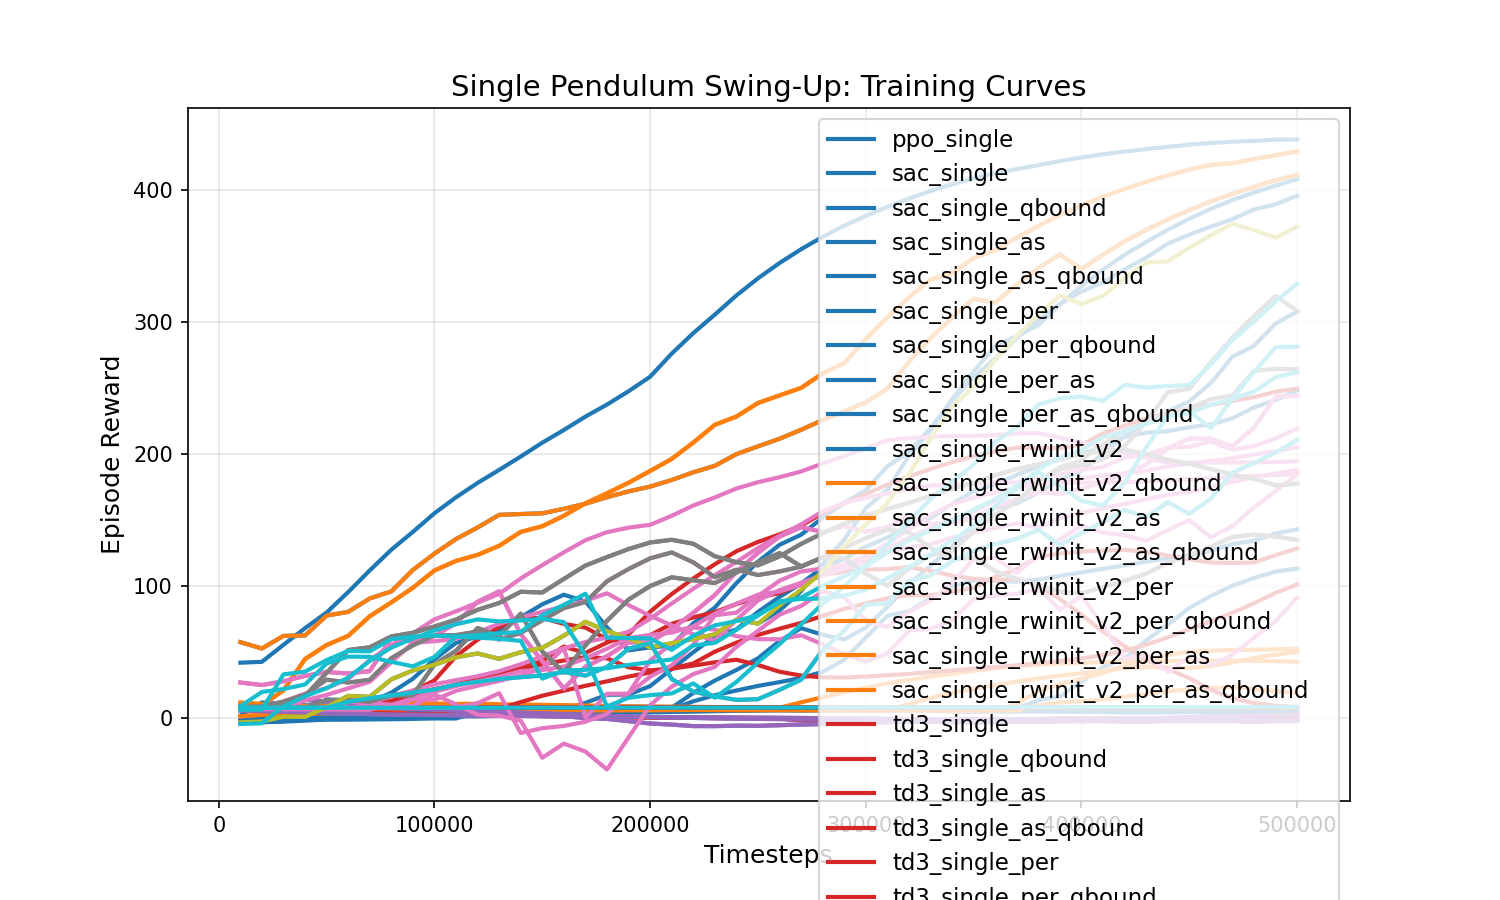
\includegraphics[width=\textwidth]{training_curves_single.png}
\caption{Training curves for all single-pendulum experiments. Raw (transparent) and smoothed (solid) mean episode rewards. SAC+QBound variants (top cluster) converge stably to $\sim$450, while TD3 variants remain mostly stuck near zero.}
\label{fig:curves_single}
\end{figure}

\begin{figure}[H]
\centering
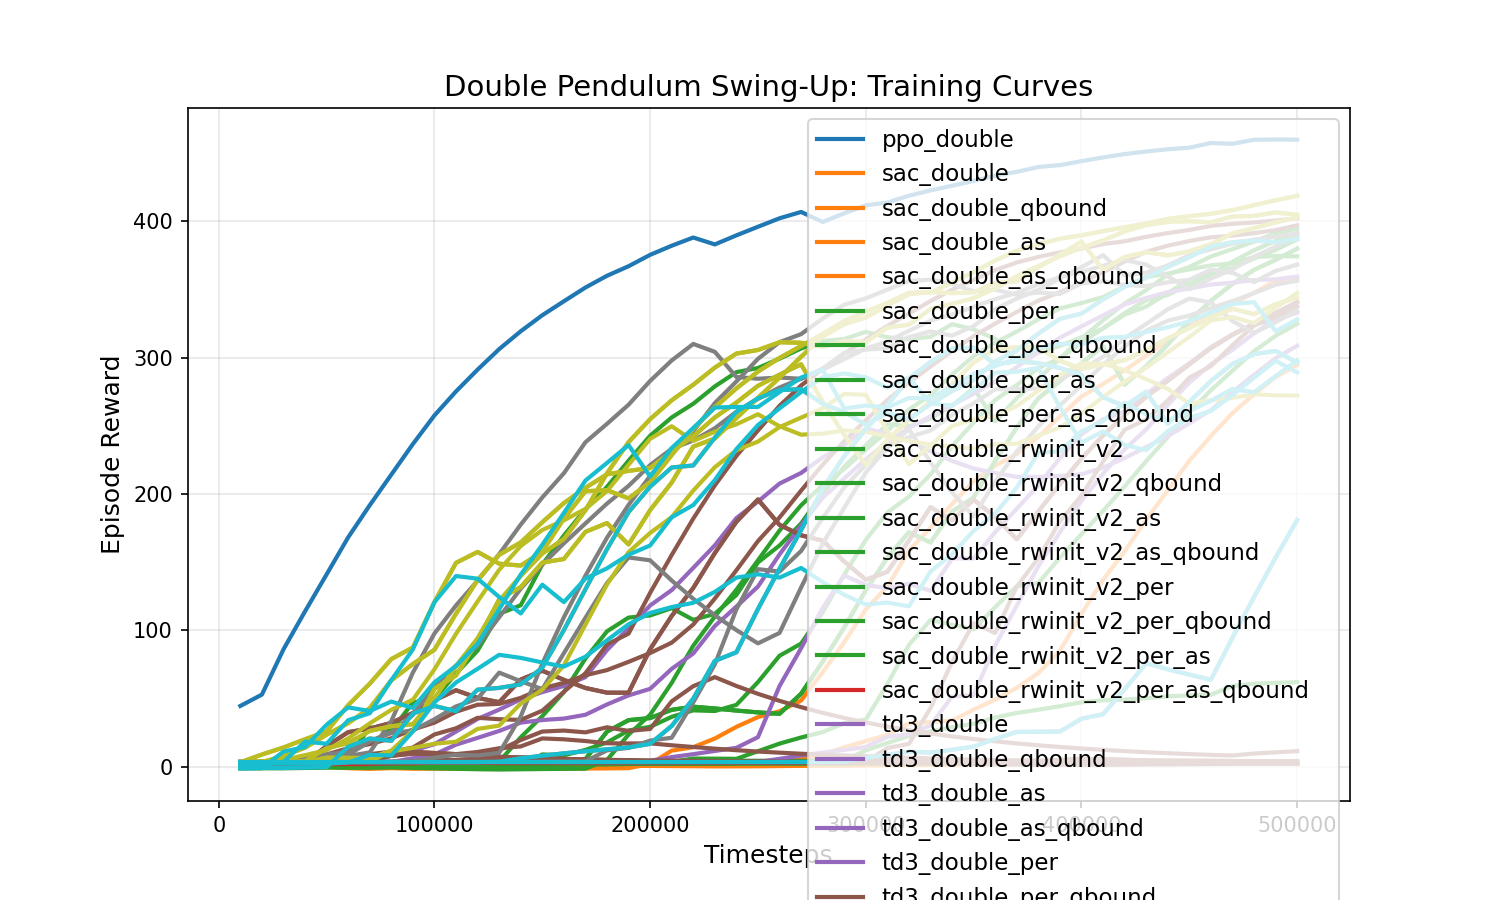
\includegraphics[width=\textwidth]{training_curves_double.png}
\caption{Training curves for all double-pendulum experiments. Most algorithms achieve $>$400 on the double pendulum, with broader separation between technique variants. DDPG and SAC configurations show the strongest performance.}
\label{fig:curves_double}
\end{figure}

\section{Analysis}

\subsection{Technique--Algorithm Interaction}

\begin{table}[h]
\centering
\caption{Effect of each technique relative to algorithm baseline.}
\begin{tabular}{lccc}
\toprule
Technique & SAC & TD3 & DDPG \\
\midrule
RWAI v2 & Strong positive & Destructive & High peak, unstable \\
PER & Moderate & Neutral & Mixed \\
AS & \textbf{Catastrophic} & \textbf{Partially rescues} & Mixed \\
QBound & \textbf{Excellent} & Neutral single, positive double (from \texttt{norm\_reward=False}) & Neutral \\
\bottomrule
\end{tabular}
\label{tab:interaction}
\end{table}

The most striking finding is the opposing effects of AS across algorithms. AS corrupts SAC's squashed Gaussian log-probability computation:
\begin{equation}
\log \pi(a|s) = \log \mu(u|s) - \sum_i \log(1 - \tanh^2(u_i))
\end{equation}
The AdaptiveGradientScaler remaps $u_i$ based on running statistics, changing the relationship between the Gaussian parameters and the tanh correction term, corrupting entropy estimates and destabilizing $\alpha$-tuning. TD3/DDPG use deterministic policies (no log-probability), so AS safely prevents tanh saturation.

\subsection{QBound as Q-Value Regularization}

QBound constrains Q-values to $[Q_{\min}, Q_{\max}]$, preventing the late-training drift that degrades SAC baselines. Since QBound requires \texttt{norm\_reward=False}, fair comparison uses the \texttt{no\_norm\_reward} baseline: most of the SAC single-pendulum gain ($312 \to 452.6$) comes from disabling reward normalization; QBound adds stability ($452.2$ vs.\ $448.3$ final). On double pendulum, QBound alone matches the \texttt{no\_norm\_reward} baseline exactly ($452.0/408.7$), but PER+QBound achieves substantially better stability ($455.7/455.7$). The mechanism is twofold: (1)~preventing Q-value inflation maintains critic accuracy; (2)~bounded Q-values keep the entropy term at consistent relative scale, stabilizing $\alpha$-tuning.

\textbf{When does QBound actually fire?} Comparing RWAI~v2+QBound against RWAI~v2 alone (a fair comparison since both use \texttt{norm\_reward=False}) reveals that results are identical across all three algorithms on both environments---QBound's clipping never activates when RWAI~v2 is present, because the well-calibrated initialization keeps Q-values within the theoretical bounds. Similarly, standalone QBound matches the \texttt{no\_norm\_reward} baseline exactly for TD3 ($8.6/8.6$ single, $429.9/429.9$ double) and DDPG ($363.7/294.1$ single, $478.0/219.8$ double), confirming that QBound's clipping mechanism never fires for these algorithms---their Q-values naturally remain within $[Q_{\min}, Q_{\max}]$. Only SAC's entropy-driven exploration pushes Q-values outside the theoretical bounds, producing the modest single-pendulum stability gain ($+3.9$ final) and the substantial PER+QBound synergy on double ($+47.0$ final).

\textbf{Is QBound risk-free?} In the fair RWAI~v2 comparisons, QBound is neutral in most combinations (identical results). However, when QBound does activate in AS-containing configurations, effects can be mixed: SAC RWAI~v2+PER+QBound on double achieves a higher peak ($463.1$ vs.\ $456.1$) but lower final ($424.7$ vs.\ $444.7$, $-20.0$) compared to RWAI~v2+PER without QBound. QBound is thus best characterized as \emph{low-risk} rather than zero-risk: it is inert when Q-values stay in range, beneficial for SAC in standard configurations, but can interact unpredictably with AS-damaged training dynamics.

\subsection{PER as Synergy Amplifier}

PER alone provides inconsistent benefits but significantly amplifies other techniques: PER + QBound (SAC: 453.5/455.7 final), PER + AS (TD3: 292.5/269.5 single), PER + RWAI v2 (SAC: 454.4/453.3). PER's TD-error-based sampling exploits the distinct error patterns created by each technique.

\subsection{The TD3 Single-Pendulum Problem}

TD3's complete failure on single pendulum (8.7 across most variants) is confirmed as a fundamental clipped-double-Q limitation:
\begin{itemize}
\item DDPG solves it (298.8)---same architecture minus double-Q
\item RWAI v1 temporarily rescues (272.4 peak)---overestimation breaks the trap
\item AS partially rescues (205.4)---tanh desaturation enables exploration
\item QBound/\texttt{no\_norm\_reward} helps TD3 double ($+41.6$ final, attributable to disabling reward normalization) but not single; PER, RWAI v2 alone do not help single
\end{itemize}

\subsection{Competitiveness with PPO}
\label{sec:ppo_benchmark}

PPO serves as the on-policy performance ceiling: $450.2/439.0$ best/final (single), $488.0/458.7$ (double). A central question is whether the investigated techniques make off-policy algorithms competitive with PPO.

\begin{table}[h]
\centering
\caption{Off-policy vs PPO benchmark. ``Gap'' is the difference in final reward relative to PPO. Positive values indicate the off-policy configuration \emph{exceeds} PPO.}
\small
\begin{tabular}{llccr}
\toprule
Algorithm & Configuration & Best & Final & Gap vs PPO \\
\midrule
\multicolumn{5}{l}{\emph{Single pendulum (PPO final: 439.0)}} \\
SAC & baseline (GC only) & 312.4 & 312.4 & $-126.6$ \\
SAC & + QBound & 453.2 & 452.2 & $\mathbf{+13.2}$ \\
SAC & + PER + QBound & 453.6 & 453.5 & $\mathbf{+14.5}$ \\
TD3 & baseline (GC only) & 8.7 & 8.7 & $-430.3$ \\
TD3 & + PER + AS & 292.5 & 269.5 & $-169.5$ \\
DDPG & baseline (GC only) & 298.8 & 298.8 & $-140.2$ \\
DDPG & + RWAI v2 + PER & 455.4 & 206.2 & $-232.8$ \\
\midrule
\multicolumn{5}{l}{\emph{Double pendulum (PPO final: 458.7)}} \\
SAC & baseline (GC only) & 434.5 & 369.9 & $-88.8$ \\
SAC & + PER + QBound & 455.7 & 455.7 & $-3.0$ \\
SAC & + RWAI v2 & 482.9 & 453.7 & $-5.0$ \\
TD3 & + PER + AS & 441.4 & 428.8 & $-29.9$ \\
DDPG & + AS & 457.9 & 457.1 & $-1.6$ \\
\bottomrule
\end{tabular}
\label{tab:ppo_gap}
\end{table}

\textbf{Key findings:} On single pendulum, SAC baselines underperform PPO by 127 points, but QBound closes this gap entirely---SAC + QBound and SAC + PER + QBound \emph{exceed} PPO by $+13$--$15$ points. TD3 remains far below PPO even with its best configuration (PER + AS: $-170$). On double pendulum, multiple off-policy configurations approach PPO-level performance: DDPG + AS ($-1.6$), SAC + PER + QBound ($-3.0$), and SAC + RWAI v2 ($-5.0$). Without the investigated techniques, off-policy algorithms are consistently inferior to PPO on these hard-exploration tasks; \emph{with} the right technique combination, SAC matches or exceeds PPO while retaining off-policy sample efficiency advantages.

\subsection{The Overestimation Spectrum}

Our results map a spectrum from harmful underestimation (TD3 default: 8.7) through beneficial moderate overestimation (DDPG default: 298.8) to harmful excessive overestimation (SAC + RWAI v1: collapse). QBound enforces a ceiling preventing the right extreme; AS addresses the left extreme by enabling exploration despite conservative Q-estimates.

\section{Practical Recommendations}

\textbf{For SAC:} Add QBound with environment-derived bounds. Consider RWAI v2 + PER for peak performance. \textbf{Never use AS with SAC.}

\textbf{For TD3:} Use PER + AS to escape exploration traps. Avoid RWAI v2. Consider DDPG as an alternative for hard-exploration tasks.

\textbf{For DDPG:} RWAI v2 for peak performance (with instability tradeoff). AS for double-pendulum stability.

\textbf{General:} Always use gradient clipping. Disable reward normalization when using QBound or RWAI v2. The optimal technique combination is algorithm-specific.

\section{Limitations}

\begin{enumerate}
\item \textbf{Single-seed evaluation:} All experiments use seed 42. Multi-seed evaluation is needed for statistical significance.
\item \textbf{Two environments:} Dense rewards in $[-0.5, 1.0]$. Generalization to sparse/negative rewards is not established.
\item \textbf{Fixed hyperparameters:} Technique interactions with different hyperparameter regimes are unknown.
\item \textbf{AS--SAC interaction:} The log-probability corruption mechanism warrants further analysis (e.g., tracking entropy coefficient dynamics).
\end{enumerate}

\section{Conclusion}

We present a comprehensive 116-experiment ablation study of five complementary techniques for off-policy deep RL. The principal findings are:

\begin{enumerate}
\item \textbf{QBound provides the most stable SAC performance.} Against the fair \texttt{no\_norm\_reward} baseline, QBound adds stability rather than raw improvement; PER + QBound achieves the highest stable finals ($453.5$ single, $455.7$ double). The headline gain ($312 \to 453$) is primarily from disabling reward normalization, which QBound requires. QBound's clipping is inert for TD3 and DDPG (Q-values naturally stay within bounds) and activates only for SAC, where entropy-driven exploration pushes estimates outside the theoretical range. QBound is low-risk---neutral when it does not fire---though it can interact unpredictably with AS-damaged training dynamics.

\item \textbf{Adaptive Gradient Scaling is catastrophic for SAC without QBound but rescues TD3}---the same technique that corrupts SAC's log-probability computation enables TD3 to partially escape exploration failure ($8.7 \to 205$). Notably, QBound partially rescues AS-damaged SAC (AS+QBound: $225/421$ single/double vs.\ pure AS: $8/3$).

\item \textbf{RWAI v2 improves SAC double pendulum} (482.9 peak) \textbf{but destabilizes TD3}. On single pendulum, RWAI v2 matches the \texttt{no\_norm\_reward} baseline (452.6), so the benefit is primarily on double. Informed initialization interacts destructively with conservative Q-estimation.

\item \textbf{PER functions as a synergy amplifier}, providing its greatest benefits when combined with QBound or AS.

\item \textbf{No single technique universally improves all algorithms.} The optimal configuration is algorithm-specific: SAC + PER + QBound, TD3 + PER + AS, DDPG + AS (double).

\item \textbf{Conservative Q-estimation harms exploration.} TD3's clipped double-Q suppresses value signals from rare high-reward transitions, causing complete failure on single pendulum while DDPG solves it.
\end{enumerate}

These results demonstrate that technique selection for off-policy RL must be algorithm-aware, and that the interaction between Q-estimation architecture and training stabilization techniques determines practical effectiveness.

\bibliographystyle{plainnat}

\begin{thebibliography}{16}

\bibitem[Haarnoja et~al.(2018)]{haarnoja2018sac}
T.~Haarnoja, A.~Zhou, P.~Abbeel, and S.~Levine.
\newblock Soft Actor-Critic: Off-Policy Maximum Entropy Deep Reinforcement Learning with a Stochastic Actor.
\newblock In \emph{ICML}, 2018.

\bibitem[Fujimoto et~al.(2018)]{fujimoto2018td3}
S.~Fujimoto, H.~van Hoof, and D.~Meger.
\newblock Addressing Function Approximation Error in Actor-Critic Methods.
\newblock In \emph{ICML}, 2018.

\bibitem[Lillicrap et~al.(2016)]{lillicrap2016ddpg}
T.~P. Lillicrap, J.~J. Hunt, A.~Pritzel, N.~Heess, T.~Erez, Y.~Tassa, D.~Silver, and D.~Wierstra.
\newblock Continuous Control with Deep Reinforcement Learning.
\newblock In \emph{ICLR}, 2016.

\bibitem[Glorot and Bengio(2010)]{glorot2010xavier}
X.~Glorot and Y.~Bengio.
\newblock Understanding the difficulty of training deep feedforward neural networks.
\newblock In \emph{AISTATS}, 2010.

\bibitem[He et~al.(2015)]{he2015kaiming}
K.~He, X.~Zhang, S.~Ren, and J.~Sun.
\newblock Delving Deep into Rectifiers: Surpassing Human-Level Performance on ImageNet Classification.
\newblock In \emph{ICCV}, 2015.

\bibitem[Saxe et~al.(2014)]{saxe2014orthogonal}
A.~M. Saxe, J.~L. McClelland, and S.~Ganguli.
\newblock Exact solutions to the nonlinear dynamics of learning in deep linear neural networks.
\newblock In \emph{ICLR}, 2014.

\bibitem[Thrun and Schwartz(1993)]{thrun1993overestimation}
S.~Thrun and A.~Schwartz.
\newblock Issues in Using Function Approximation for Reinforcement Learning.
\newblock In \emph{Connectionist Models Summer School}, 1993.

\bibitem[van Hasselt(2010)]{vanhasselt2010doubleq}
H.~van Hasselt.
\newblock Double Q-learning.
\newblock In \emph{NeurIPS}, 2010.

\bibitem[Kumar et~al.(2020)]{kumar2020cql}
A.~Kumar, A.~Zhou, G.~Tucker, and S.~Levine.
\newblock Conservative Q-Learning for Offline Reinforcement Learning.
\newblock In \emph{NeurIPS}, 2020.

\bibitem[Sutton and Barto(2018)]{sutton2018rl}
R.~S. Sutton and A.~G. Barto.
\newblock \emph{Reinforcement Learning: An Introduction}.
\newblock MIT Press, 2018.

\bibitem[Schulman et~al.(2017)]{schulman2017ppo}
J.~Schulman, F.~Wolski, P.~Dhariwal, A.~Radford, and O.~Klimov.
\newblock Proximal Policy Optimization Algorithms.
\newblock \emph{arXiv:1707.06347}, 2017.

\bibitem[Raffin et~al.(2021)]{raffin2021sb3}
B.~Raffin, A.~Hill, A.~Gleave, A.~Kanervisto, M.~Ernestus, and N.~Dormann.
\newblock Stable-Baselines3: Reliable Reinforcement Learning Implementations.
\newblock \emph{JMLR}, 2021.

\bibitem[Hollenstein et~al.(2022)]{hollenstein2022noise}
J.~Hollenstein, S.~Auddy, M.~Saveriano, E.~Renaudo, and J.~Piater.
\newblock Action Noise in Off-Policy Deep Reinforcement Learning: Impact on Exploration and Performance.
\newblock \emph{arXiv:2206.03787}, 2022.

\bibitem[Eberhard et~al.(2023)]{eberhard2023pink}
O.~Eberhard, J.~Hollenstein, C.~Pinneri, and G.~Martius.
\newblock Pink Noise Is All You Need: Colored Noise Exploration in Deep Reinforcement Learning.
\newblock In \emph{ICLR}, 2023.

\bibitem[Raffin(2020)]{raffin2020gsde}
A.~Raffin.
\newblock Generalized State-Dependent Exploration for Deep Reinforcement Learning in Robotics.
\newblock \emph{arXiv:2005.05719}, 2020.

\bibitem[Schaul et~al.(2016)]{schaul2016per}
T.~Schaul, J.~Quan, I.~Antonoglou, and D.~Silver.
\newblock Prioritized Experience Replay.
\newblock In \emph{ICLR}, 2016.

\bibitem[Gebrekidan(2025a)]{gebrekidan2025qbound}
T.~Z. Gebrekidan.
\newblock QBound: Q-Value Bounding for Off-Policy Deep Reinforcement Learning.
\newblock \url{https://github.com/TesfayZ/QBound}, 2025.

\bibitem[Gebrekidan(2025b)]{gebrekidan2025as}
T.~Z. Gebrekidan.
\newblock Gradient Asymmetry and Activation Saturation in Deep Reinforcement Learning.
\newblock \url{https://github.com/TesfayZ/gradient_asymetry_AND_activation_saturation}, 2025.

\end{thebibliography}

\end{document}
